Before the training or inference processes can take place a feature selection should be performed and for this experiment a stepwise regression algorithm with five steps forward and three steps backward was used. From 196 available features a set of 16 features was chosen. The optimal set is combination of features representing colours of superpixels from the the already defined grid as well as percentage of red, green and blue superpixels in the neighbourhood of a given grid point. Figures \ref{fig:nonlinear_noise_free_features_colour} and \ref{fig:nonlinear_noise_free_features_percentage} present visualisations of which features were chosen by the selection algorithm.
\begin{figure}[ht]
    \centering
    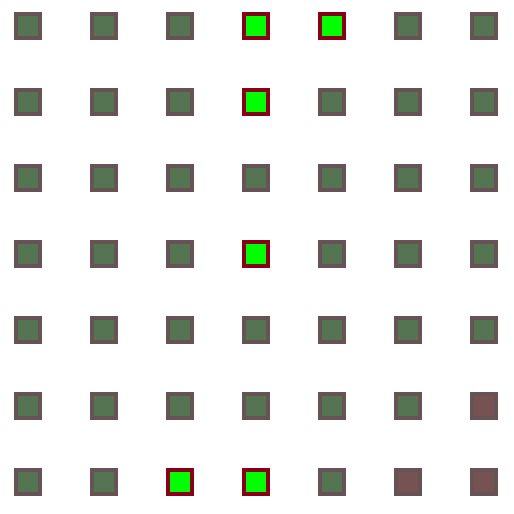
\includegraphics[width=0.5\textwidth]{nonlinear_noise_free/features/grid_colour_chosen.png}
    \caption{Chosen grid colour features for experiments on noise-free data}
    \label{fig:nonlinear_noise_free_features_colour}
\end{figure}
\begin{figure}[ht]
    \centering
    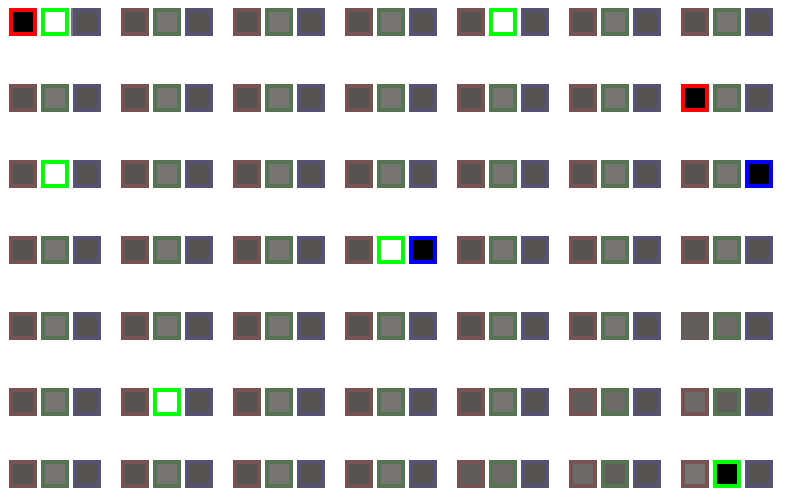
\includegraphics[width=\textwidth]{nonlinear_noise_free/features/grid_colour_percentage_chosen.png}
    \caption{Chosen grid neighbour colour percentage features for experiments on noise-free data.}
    \label{fig:nonlinear_noise_free_features_percentage}
\end{figure}

First figure depicts neighbour colour features for a sample superpixel, and the second shows neighbour colour percentage features. The way of feature presentation is the same as in the previous experiment. Features which were not chosen are covered by an extra semitransparent layer, while those which form the final feature set are left unchanged.

Optimal features were selected based on a validation set of generated images, hence, to check whether the selection was indeed optimal an extra test was performed. For images from the testing set, which were not used during the feature selection process, the conditional probability $p(y|x)$ was computed for every label and for the selected feature set for every test image. The resulting probabilities for three sample images, each with a main object of a different shape, are presented in a visual way in figure \ref{fig:noise_free_fi1}. In the first row an original image is depicted and the next four rows show calculated conditional probabilities, one per each label. A colour of the superpixel represents a probability that this superpixel will be assigned to the given class. The higher is this probability the lighter is the colour. Hence, when a superpixel has 100\% chances of being assigned to some class, it will be white, and conversely for 0\% of probability such pixel will be black. 
\begin{center}
 \renewcommand{\arraystretch}{4}
    \begin{tabular}{cccc}
        \textit{test image} &
        \fcolorbox{black}{white}{\includegraphics[align=c,width= 0.22\textwidth]{nonlinear_noise_free/fi_1/1/image.png}} &
        \fcolorbox{black}{white}{\includegraphics[align=c,width= 0.22\textwidth]{nonlinear_noise_free/fi_1/2/image.png}} &
        \fcolorbox{black}{white}{\includegraphics[align=c,width= 0.22\textwidth]{nonlinear_noise_free/fi_1/3/image.png}}  \\
        \textit{label 0} &
        \fcolorbox{black}{white}{\includegraphics[align=c,width= 0.22\textwidth]{nonlinear_noise_free/fi_1/1/label_0.png}} &
        \fcolorbox{black}{white}{\includegraphics[align=c,width= 0.22\textwidth]{nonlinear_noise_free/fi_1/2/label_0.png}} &
        \fcolorbox{black}{white}{\includegraphics[align=c,width= 0.22\textwidth]{nonlinear_noise_free/fi_1/3/label_0.png}} \\
        \textit{label 1} &
        \fcolorbox{black}{white}{\includegraphics[align=c,width= 0.22\textwidth]{nonlinear_noise_free/fi_1/1/label_1.png}} &
        \fcolorbox{black}{white}{\includegraphics[align=c,width= 0.22\textwidth]{nonlinear_noise_free/fi_1/2/label_1.png}} &
        \fcolorbox{black}{white}{\includegraphics[align=c,width= 0.22\textwidth]{nonlinear_noise_free/fi_1/3/label_1.png}} \\
        \textit{label 2} &
        \fcolorbox{black}{white}{\includegraphics[align=c,width= 0.22\textwidth]{nonlinear_noise_free/fi_1/1/label_2.png}} &
        \fcolorbox{black}{white}{\includegraphics[align=c,width= 0.22\textwidth]{nonlinear_noise_free/fi_1/2/label_2.png}} &
        \fcolorbox{black}{white}{\includegraphics[align=c,width= 0.22\textwidth]{nonlinear_noise_free/fi_1/3/label_2.png}} \\
        \textit{label 3} &
        \fcolorbox{black}{white}{\includegraphics[align=c,width= 0.22\textwidth]{nonlinear_noise_free/fi_1/1/label_3.png}} &
        \fcolorbox{black}{white}{\includegraphics[align=c,width= 0.22\textwidth]{nonlinear_noise_free/fi_1/2/label_3.png}} &
        \fcolorbox{black}{white}{\includegraphics[align=c,width= 0.22\textwidth]{nonlinear_noise_free/fi_1/3/label_3.png}}
    \end{tabular}
     \captionof{figure}{Visual representation of conditional probabilities $p(y|x)$ for three sample noise-free images.}
    \label{fig:noise_free_fi1}
\end{center}

In presented images it is visible that the algorithm has no problem in assigning proper classes to green and blue regions. The difficulty of the task lies in labelling objects into classes 0 and 3, as the only difference between objects of those classes is their shape. For these classes, the resulting probability is smaller than 100\%, therefore, there are some superpixels with different shades of grey. 

The presented probabilities form a base of computation of unary potential. If for some regions, the resulting probabilities for label 0 and 3 are more or less equal, some noised classifications may occur. In such situations, a pairwise potential is needed to ensure that neighbouring pixels from the same object will be assigned to the same class.